\chapter{Optimization of Stirling engine array}

\section{Connection types of SEA}
\label{sec:connectionTypes}
For a single Stirling engine, the heat transfer processes between fluids and engine are independent and irrelevant with the directions of the flows, which means the efficiency and power are not affected by the direction of fluids. However, for an SEA, the connection type will affect the temperature profiles through the array and the specific work production, both of which will determine the efficiency and power of the SEA. It is practically significant to investigate the influence of connection type of an SEA on its performance. Using parallel flow, on the one hand, will reduce the flow rate of the fluid, which will reduce the power of each engine; however, on the other hand, will take the advantage of higher inlet heating fluid temperature (or lower inlet cooling fluid temperature), which may increase the power of each engine. Using serial flow, on the one hand, will increase the flow rate of the fluid, which will increase the power of each engine; however, on the other hand, the inlet heating fluid temperature reduces with the flow direction (or the inlet cooling fluid temperature increases with the flow direction), which leads to lower engine power along the flow direction. Using the same order will lead to largest fluid temperature difference (temperature difference of the heating and cooling fluids) at the first engines and smallest fluid temperature difference at the last engines. Using the reverse order will lead to more averaged fluid temperature differences of each engine. For a heat exchanger, the reverse order (counterflow), which leads to a smaller fluid temperature difference, has a better heat transfer effect for its lower exergy loss. However, for a Stirling engine, the smaller fluid temperature difference leads to lower performance due to the lower temperature difference of the working gas in the hot space and cold space. To find out the influence of connection types on the performance of SEA, it is essential to classify the connection types.

Five basic connection types of SEA are summarized according to the direction-irrelevant feature of Stirling engine, as shown in \autoref{fig:SEA}. Type 1 is parallel flow, Type 2 is serial flows in the same order, Type 3 is serial flows in the reverse order, Type 4 is heating fluid in serial flow and cooling fluid in parallel flow and Type 5 is heating fluid in parallel flow and cooling fluid in serial flow. All other connection types are the combination of these five basic connection types. For instance, an SEA in \autoref{fig:SEA_eg} is the combination of Type 2 and Type 4. 
%Besides, in the tradition form of solar dish system, Stirling engines are put on the focus points of the dish collectors, which can be considered as a particular case of Type 1.

\begin{figure}[htbp]
\centering
	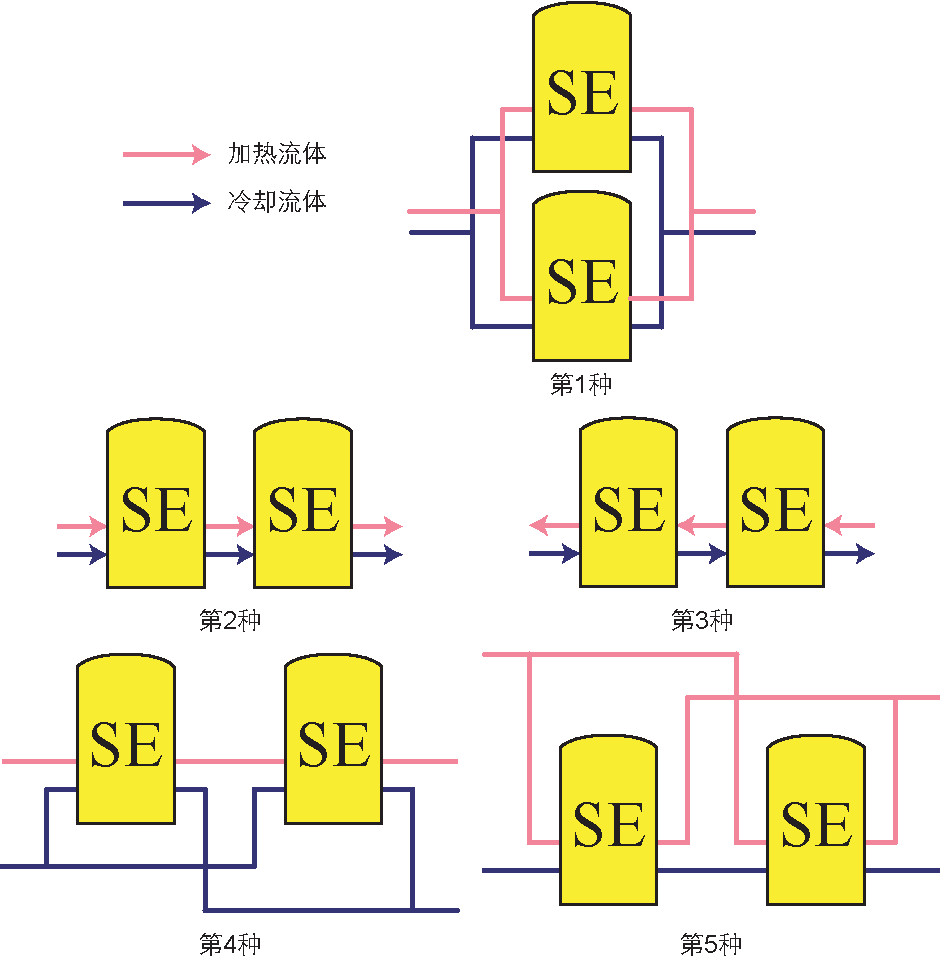
\includegraphics[width = 0.7\columnwidth]{fig/BasicSEA}
	\caption{Five basic connection types of SEA}
	\label{fig:SEA}
\end{figure}

\begin{figure}[htbp]
\centering
	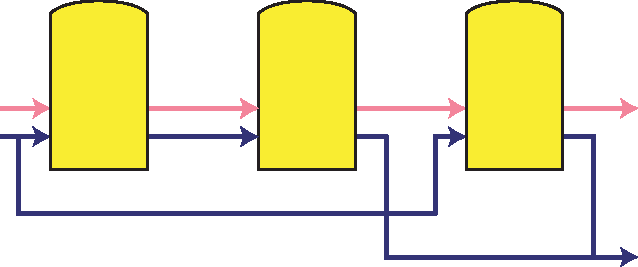
\includegraphics[width = 0.5\columnwidth]{fig/SEA_eg}
	\caption{An instance of connection type of an SEA}
	\label{fig:SEA_eg}
\end{figure}

\section{Modeling of the SEAs}

As mentioned in \autoref{sec:connectionTypes}, there are five basic connection types for an SEA. All other connection types are the combination of these five basic connection types. This thesis investigates the five basic connection types.

To determine the performance of an SEA, models of all the Stirling engines need to be built depending on their thermodynamic characteristic. Stirling engines are chosen to have the same parameters including the same speed $s_{se}$. This is a reasonable assumption when using SEA for power generation, where the output power frequency should be constant. The speed of Stirling engine can be calibrated by speed controller system~\cite{Hooshang2016}. To eliminate interference of other factors, heating and cooling fluids are chosen to have same parameters for different connection types of SEAs. To clearly find out the performance differences of different SEAs, large temperature differences of the heating/cooling fluids after heat exchange with the engines are preferred. Air is chosen as the cooling fluid instead of commonly used water to avoid small temperature rise and evaporation in the cooling process. Design parameters of Stirling engines are the same as shown in \autoref{tab:GPU3parameters}. Other parameters of Stirling engines and heating/cooling fluids in SEAs are shown in \autoref{tab:parameters}. Rotation speed of the engines and mean effective pressure are chosen to be 25$\,\mathrm{Hz}$ and 5$\,\mathrm{MPa}$ respectively to get the best Stirling engine model for performance prediction, as pointed in \autoref{sec:modelValidation}.

\begin{table}[htbp]
	\caption{Parameters of SEA models}
	\centering
	\begin{tabular}{cccc}
		\toprule
		Parameter		&	Value	& Parameter	&	Value\\
		\midrule
		Heating fluid	&	Air		&	$\dot{m}_h$	&	0.4\,kg/s\\
		Cooling fluid	&	Air	&	$T_{i,h}$	&	1000\,K\\
		$n_{se}$	&	6	&	$p_{i,h}$	&	5$\times$10$^5$\,Pa\\
		$s_{se}$	&	25\,Hz	&	$\dot{m}_c$	&	0.4\,kg/s\\
		$p_{se}$		&	5\,MPa	&	$T_{i,c}$	&	300\,K\\
		$U_hA_h$	&	180\,W/K	&	$p_{i,c}$	&	5$\times$10$^5$\,Pa\\
		$U_cA_c$		&	180\,W/K	&&\\
		\bottomrule
	\end{tabular}
	
	\label{tab:parameters}
\end{table}

In an SEA, there are 2 flows as shown in \autoref{fig:SEA}. In a serial flow, each engine's mass flow rate is $\dot{m}$, and from the flow's direction, for $2\leqslant{}x\leqslant{}n_{se}$, 
\begin{equation}
	T_{i,x} = T_{o,x-1}
	\label{Eq:T_serial}
\end{equation}
In a parallel flow, each engine's mass flow is $\dot{m}/n_{se}$, for $2\leqslant{}x\leqslant{}n_{se}$,
\begin{equation}
	T_{i,x} = T_{i,h}
	\label{Eq:T_parallel}
\end{equation}

According to the equations (\autoref{Eq:T_h}$\sim$\autoref{Eq:T_parallel})
, there are $6n_{se} - 2$ equations for $6n_{se}$ parameters for $n_{se}$ engines. Other parameters of an SEA can be calculated by the given inlet temperature of the heating and cooling fluids. The efficiency and power of each engine can be obtained from \autoref{Eq:eta} and \autoref{Eq:P}. The total efficiency and power of SEA can be obtained from powers of engines and outlet properties of the fluids.

MATLAB is used as the programming tool to build the models of SEAs, and CoolProp is used to provide fluid properties for MATLAB program. Five basic SEA models composed of the aforementioned Stirling engines and fluids are built. To compare SEA connection types under various conditions, several parameters are investigated to find out their effects on SEA performance.

\begin{figure}[htbp]
\centering
	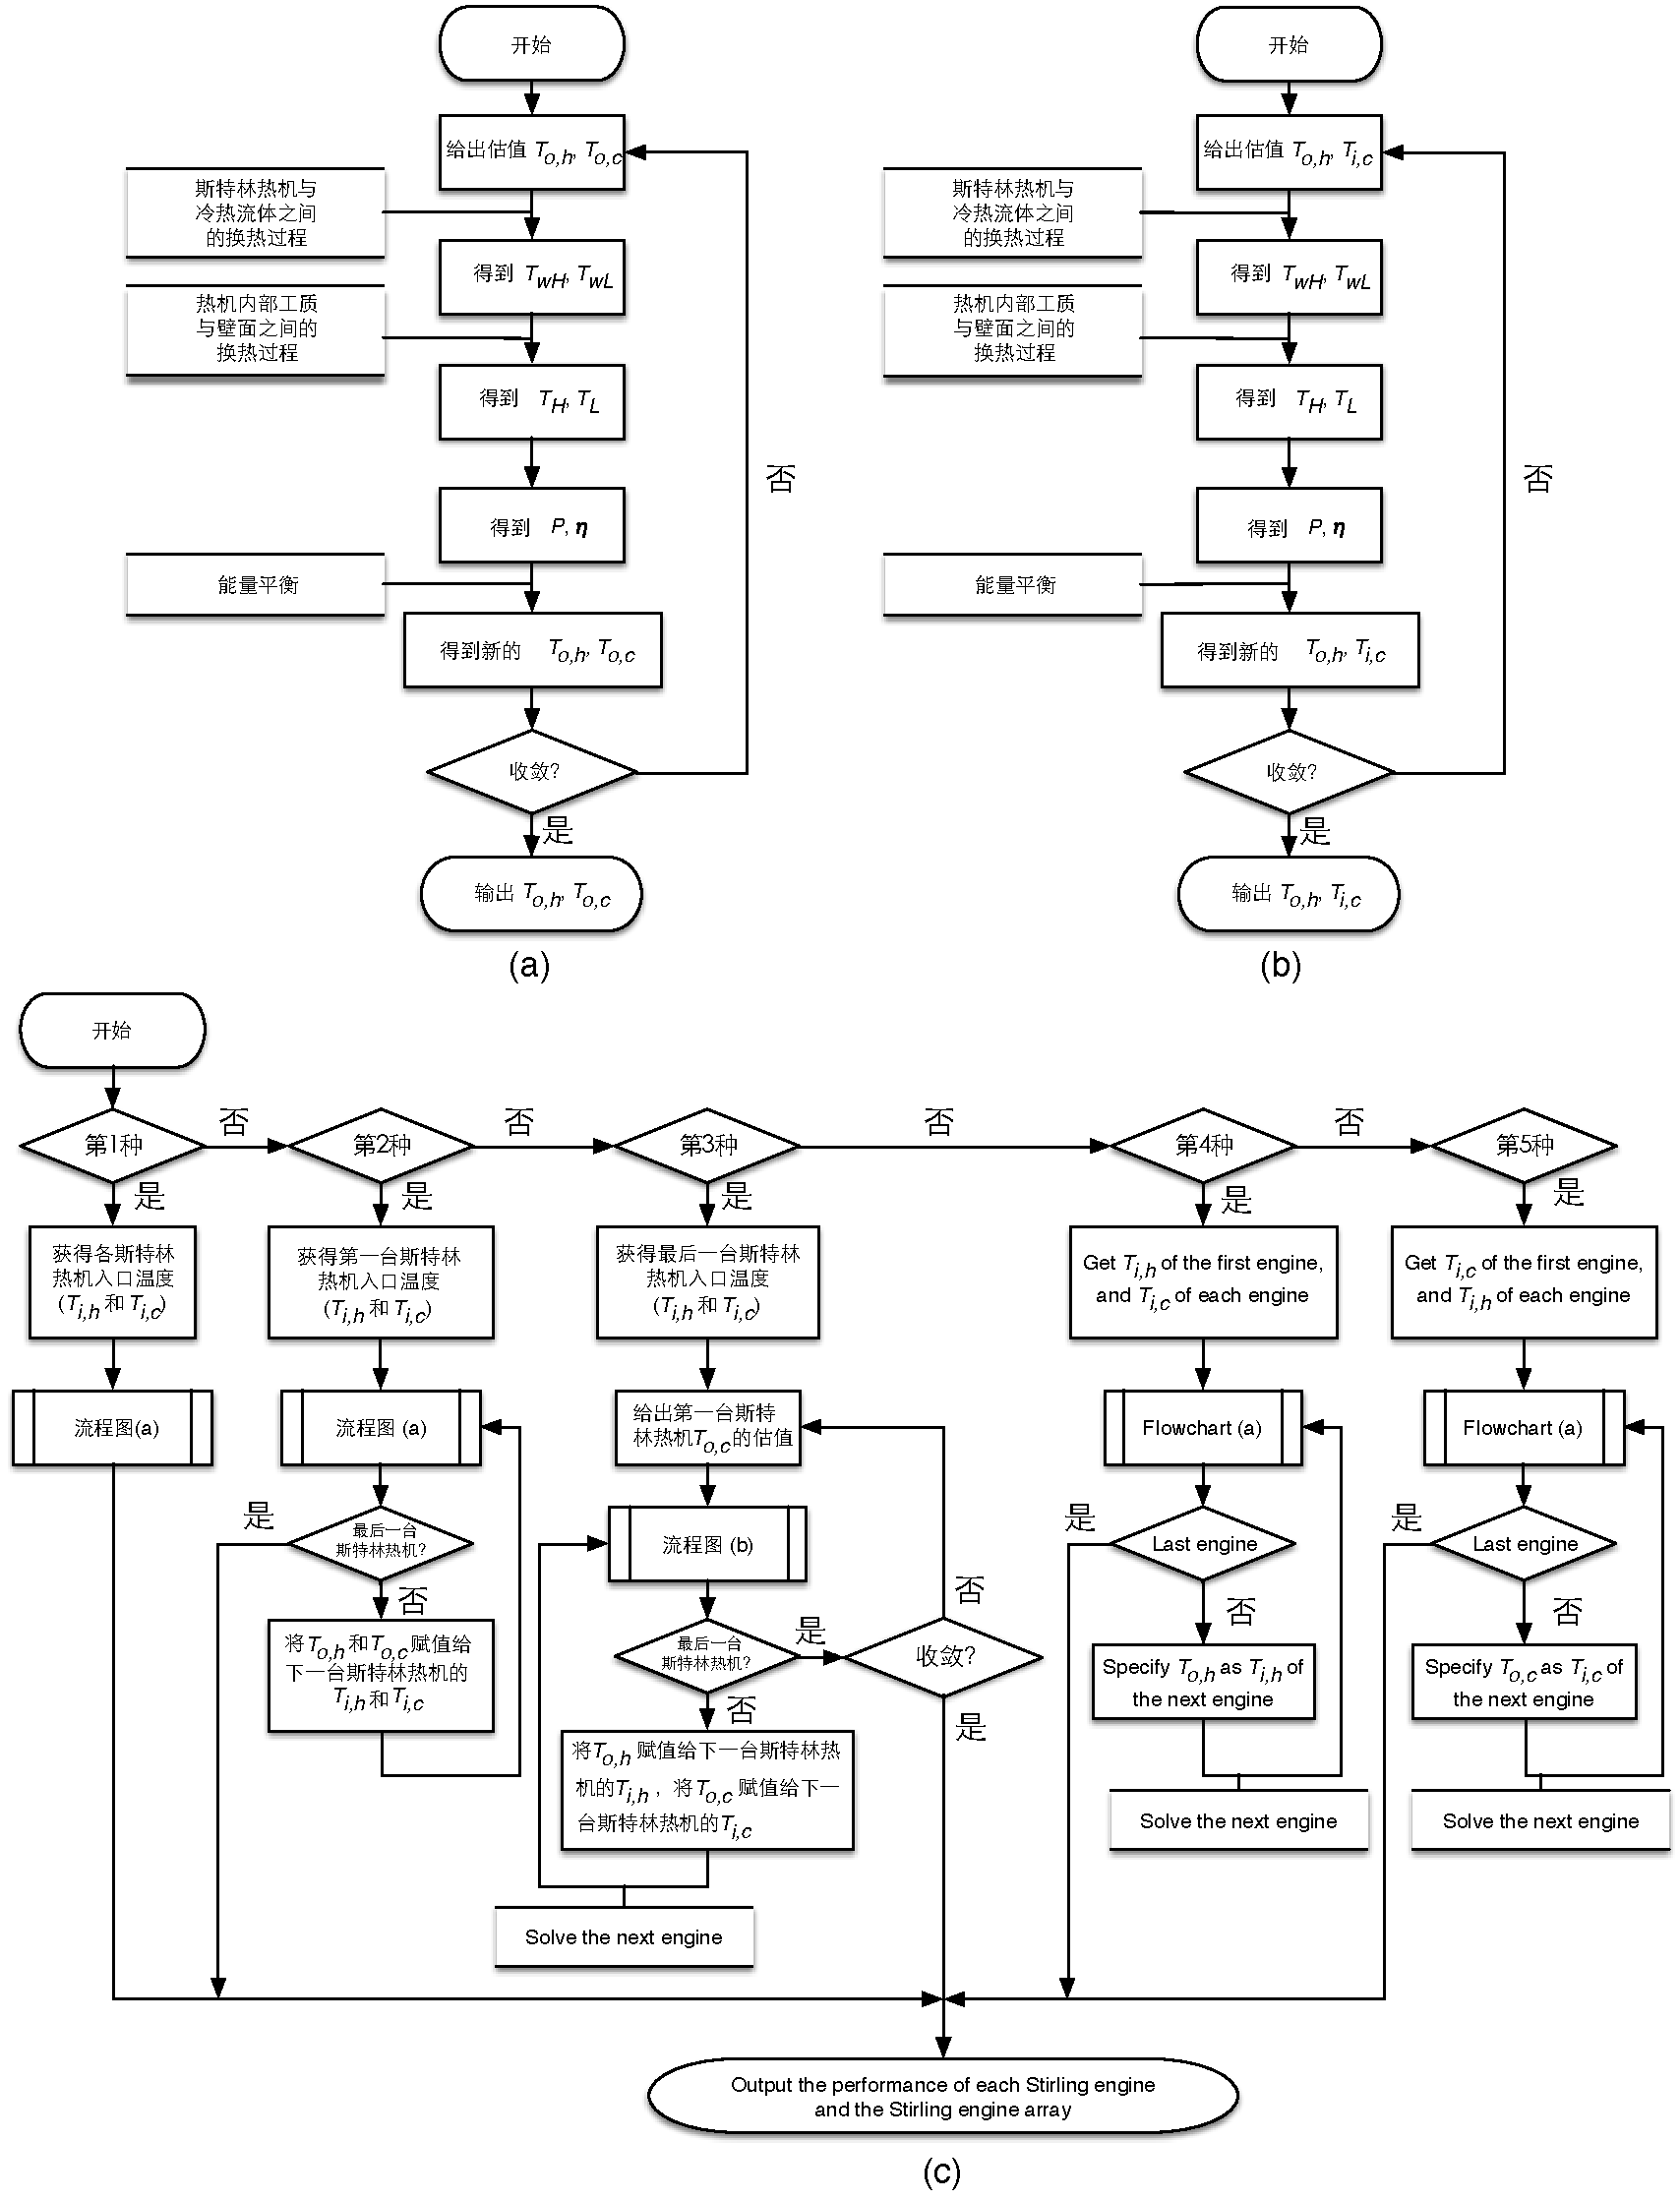
\includegraphics[width = 1.0\columnwidth]{fig/FlowChart}
	\caption{Flowcharts of the SEA model for performance analysis of the SEAs}
	\label{fig:Flowchart}

\end{figure}

\autoref{fig:Flowchart} shows the solution algorithm of the SEA model. Flowchart (a) shows the algorithm to solve a Stirling engine known inlet parameters of the fluids. Flowchart (b) shows the algorithm to solve a Stirling engine known inlet parameters of heating fluid and outlet parameters of cooling fluid. Flowchart (c) shows the algorithm to solve the SEA model iteratively depending on different connection types. The levenberg-marquardt algorithm is applied to numerically solve the non-linear equations in the flowcharts.

\section{Result analysis}
%The objective of this study is to investigate SEA performance difference of different connection types. Therefore, 

SEA models with specified parameters in \autoref{tab:parameters} are built and calculated. Results of the performances of the SEAs are shown in \autoref{tab:result}, it can be found that under specified parameters Type 3 has the highest efficiency and output power, while Type 1 has the lowest efficiency and output power.

\begin{table}[htbp]
	\caption{Results of SEA models under specified parameters}
	\centering
	\begin{tabular}{cccc}
		\toprule
		Parameter		&	Value	&	Parameter		&	Value\\
		\midrule
		$\eta_1$	&	0.2215	&	$P_1$		&	8022\,W\\
		$\eta_2$	&	0.2273	&	$P_2$		&	8483\,W\\
		$\eta_3$	&	0.2277	&	$P_3$		&	8512\,W\\
		$\eta_4$	&	0.2227	&	$P_4$		&	8116\,W\\
		$\eta_5$	&	0.2263	&	$P_5$		&	8399\,W\\		
		\bottomrule
	\end{tabular}
	\label{tab:result}
\end{table}

\subsection{Effects of $T_{i,h}$}

\begin{figure}[htpb]
\centering
	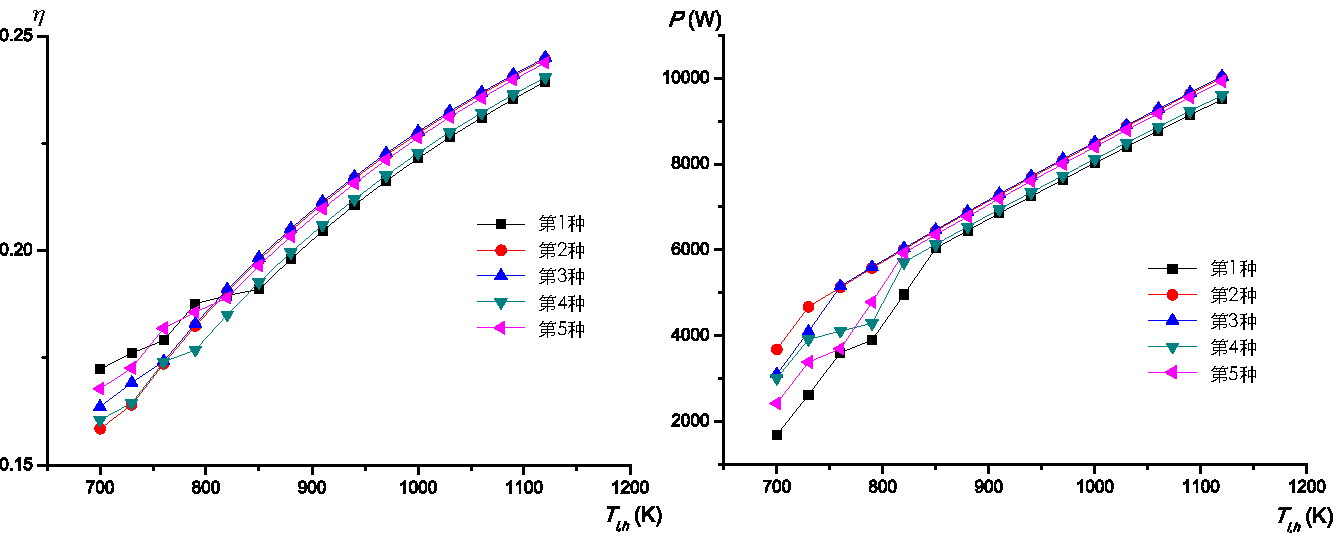
\includegraphics[width = 0.9\columnwidth]{fig/T_ih}
	\caption{Influence of $T_{i,h}$ on efficiency and power of SEA}
	\label{fig:Ti_h}
\end{figure}
According to Carnot cycle efficiency formula, the temperature of heating fluid determines the efficiency of Stirling engine array. For a Stirling engine, lower temperature heating fluid leads to a lower efficiency. The efficiency and output power may drop to 0 due to its insufficient heating fluid temperature to drive the engine.

Curves of performance of SEAs and $T_{i,h}$ are shown in \autoref{fig:Ti_h}.
As it is shown, with the increase of $T_{i,h}$, both $\eta$ and $P$ increase for all SEAs. For some types of SEA, when $T_{i,h}$ is lower than a critical temperature, some of the engines in the SEA will not work. In such situations, reduce the number of operating engines is a way to increase the total output power of the SEA. This strategy is used in the situation in \autoref{fig:Ti_h} when $T_{i,h}$ is low. Turning points on the $\eta$-$T_{i,h}$, $P$-$T_{i,h}$ curves shows the use of this strategy. The data points in the figure record the performance of the SEA with maximum output power under given conditions. 
For example, in SEA of Type 1, when $T_{i,h}$ is  820\,K, if no engines is removed from the SEA, all the engines will stop due to the low inlet fluid temperature. Remove one engine out of the system will reduce the operating number of the engines from 6 to 5, and it will increase the inlet flow rate for each engine. This will make the remaining 5 engines work again and achieve the maximum output power under the condition of $T_{i,h} = 820\,\mathrm{K}$. $820\,\mathrm{K}$ is a critical temperature for Type 1, and a turning point at 820\,K can be found on the $\eta$-$T_{i,h}$, $P$-$T_{i,h}$ curves of Type 1 in \autoref{fig:Ti_h}. 
%Multiple turning points on one curve means different engines in the SEA stop working from different temperatures.

From the curves in \autoref{fig:Ti_h}, it can be concluded that Type 2 and Type 3 have the best performance, and Type 2 has the best adaptability for lower $T_{i,h}$. All engines in Type 2 work from 730\,K.

\subsection{Effects of $\dot{m}c_p$}

According to \autoref{Eq:q_h}, \autoref{Eq:q_c}, $\dot{m}c_p$ (both $\dot{m}_hc_{p,h}$ and $\dot{m}_cc_{p,c}$) will affect the heat transfer process, which is one of the vital factor for the performance of SEA.


\begin{figure}[htbp]
\centering
	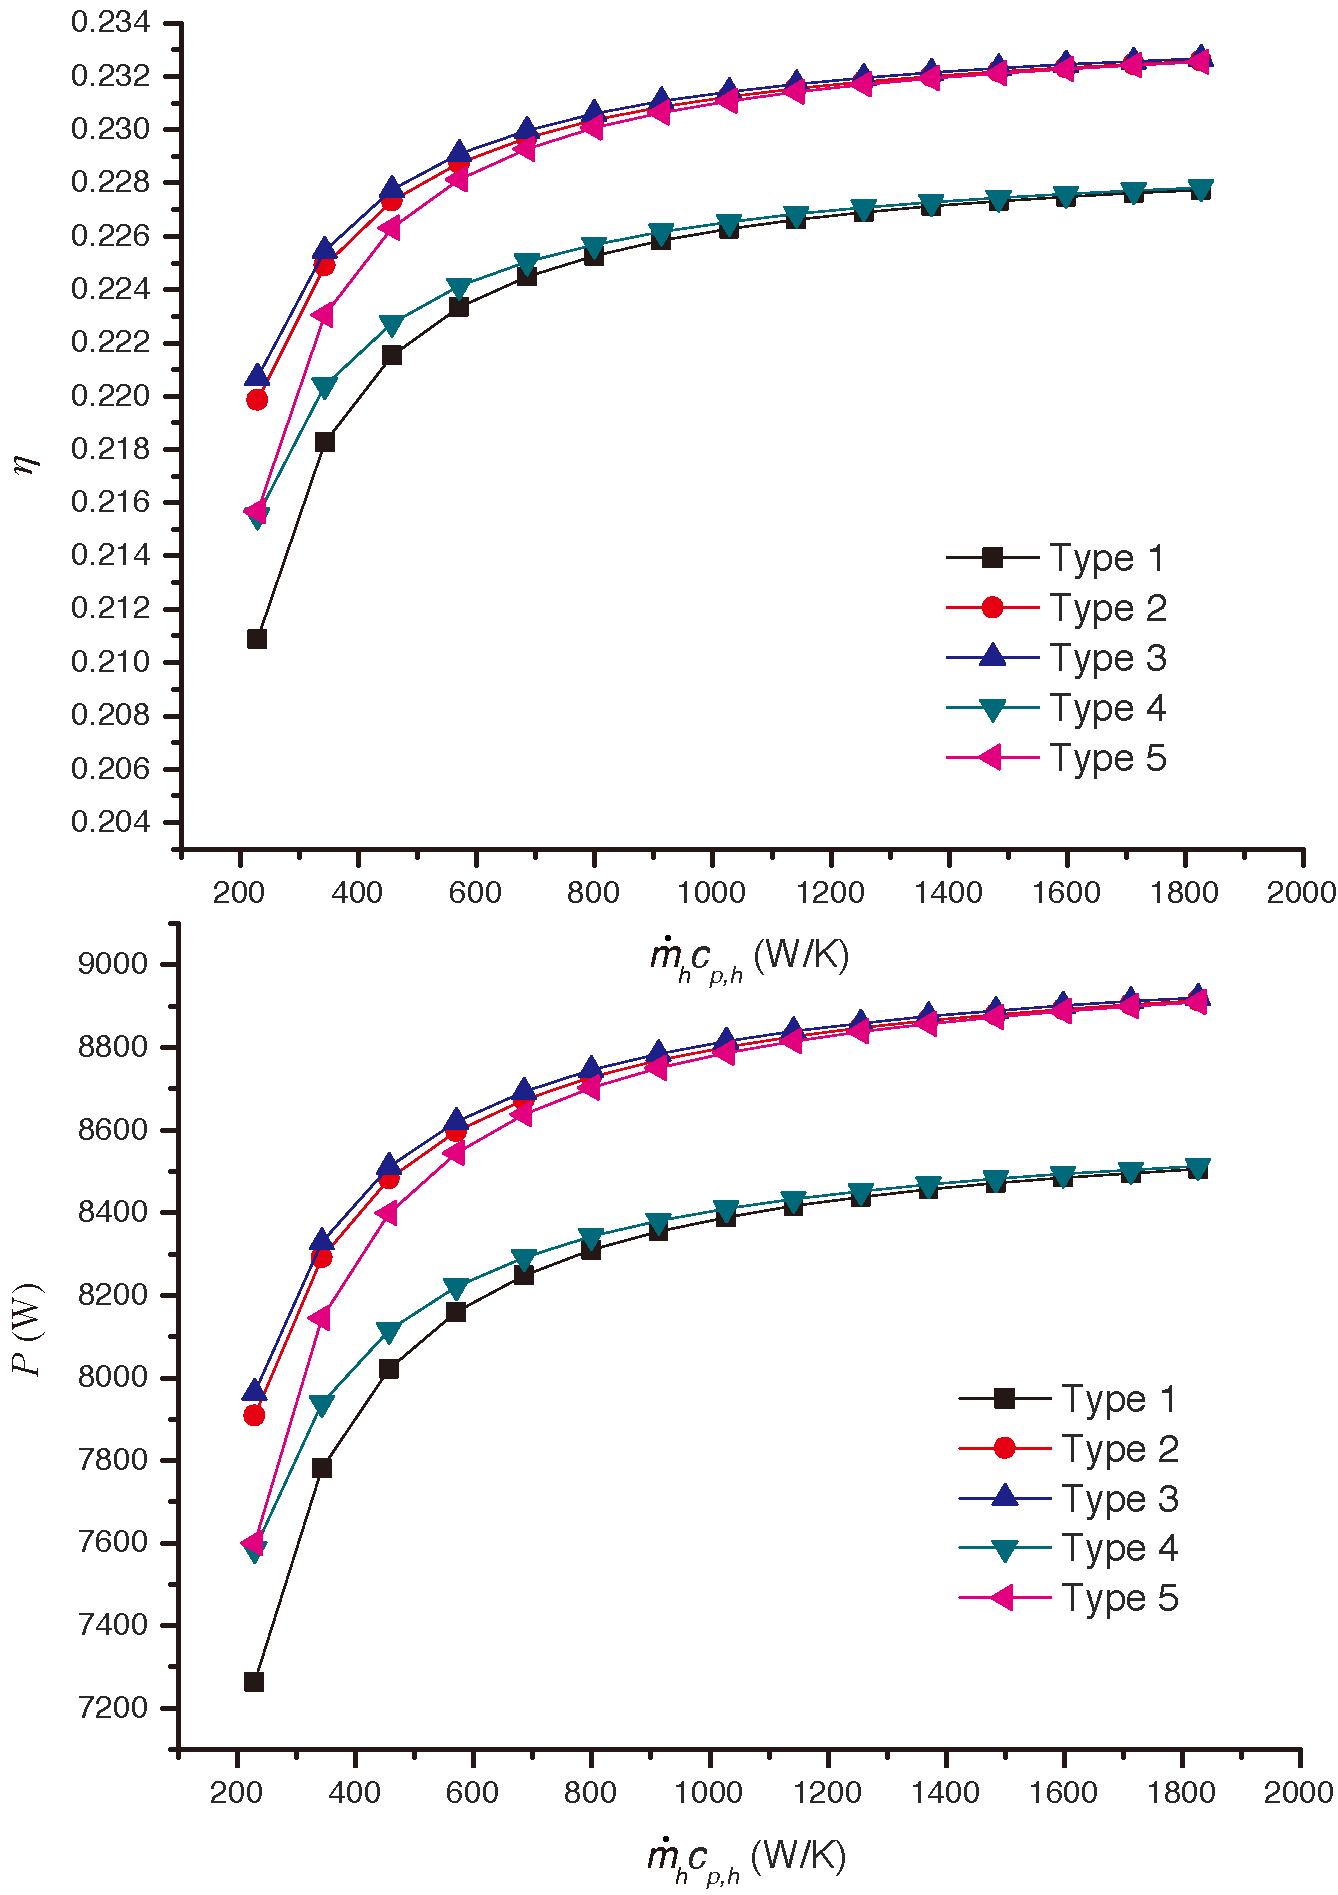
\includegraphics[width = 0.7\columnwidth]{fig/qm_hcp_h}
	\caption{Influence of $\dot{m}_hc_{p,h}$ on efficiency and power of SEA}
	\label{fig:qm_hcp_h}
\end{figure}

Curves of performance of SEAs of different $\dot{m}_hc_{p,h}$ are shown in \autoref{fig:qm_hcp_h}.
%For a connection type of SEA, $\dot{m}_hc_{p,h}$ has little effect on the performance of the SEA if it is big enough to drive the engines. This means increase the mass flow rate of heating fluid will not increase the efficiency and power of SEA significantly. 
For a large $\dot{m}_hc_{p,h}$ ($>$ 800 W/K), Type 2 , Type 3 and Type 5 have similar performance, which can be interpreted as the cooling fluid has the same properties for the two types of SEAs, and for a large $\dot{m}_hc_{p,h}$, the heating fluid has similar effect after diverged. Similar performance of Type 1 and Type 4 can be also interpreted for the same reason.

\begin{figure}[htbp]
\centering
	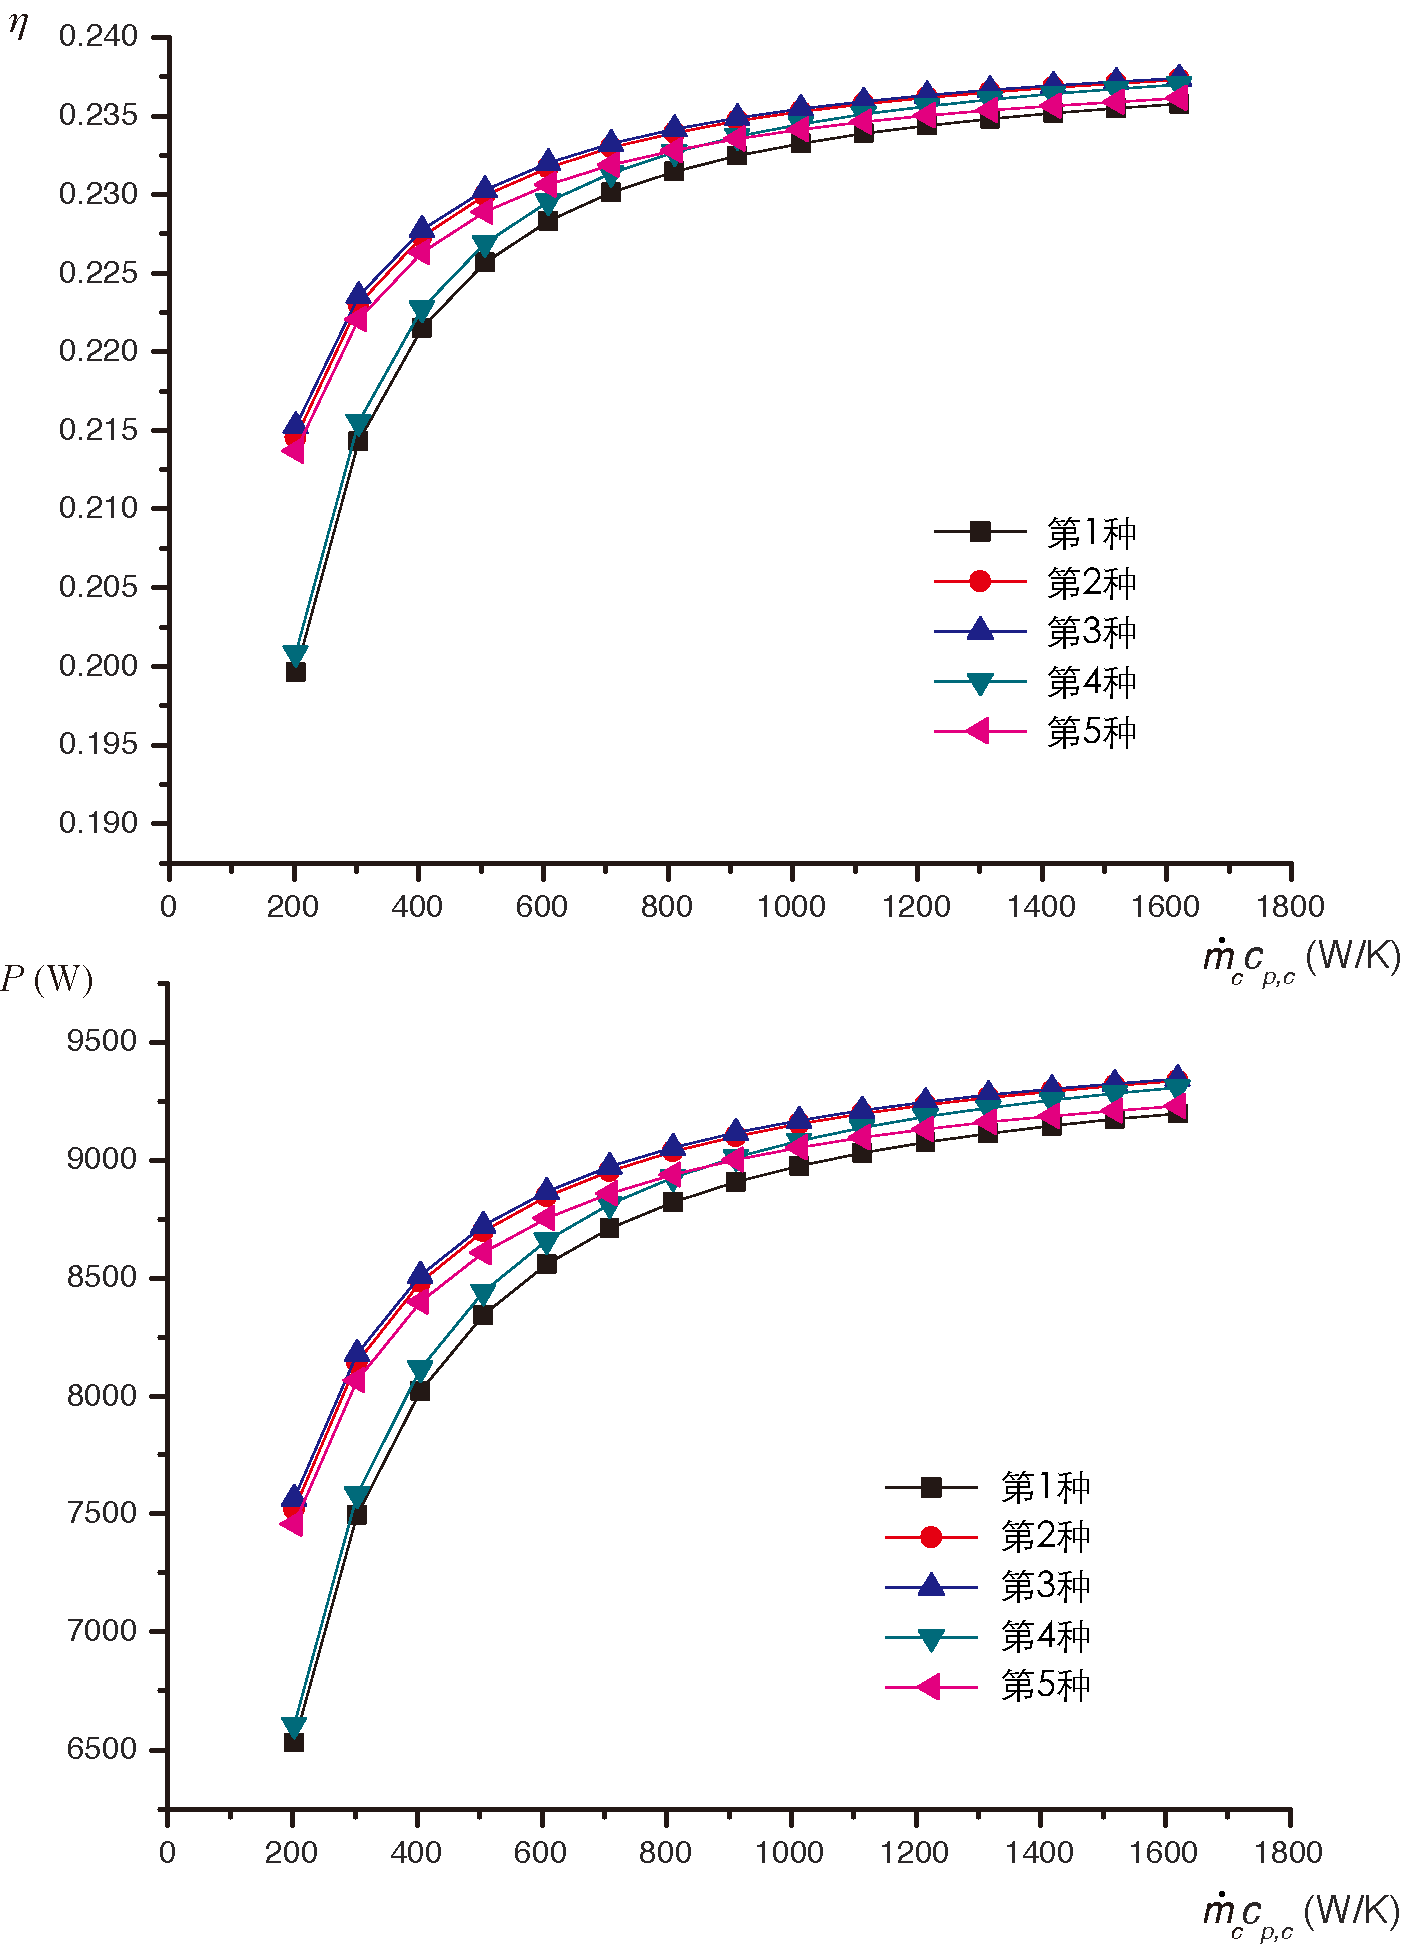
\includegraphics[width = 0.7\columnwidth]{fig/qm_ccp_c}
	\caption{Influence of $\dot{m}_cc_{p,c}$ on efficiency and power of SEA}
	\label{fig:qm_ccp_c}
\end{figure}

Curves of performance of SEAs of different $\dot{m}_cc_{p,c}$ are shown in \autoref{fig:qm_ccp_c}. For a connection type of SEA, the performance improves with the increase of $\dot{m}_cc_{p,c}$. For a large $\dot{m}_cc_{p,c}$ ($>$ 800 W/K), Type 2 and Type 3 have similar performance, which means the flow order doesn't affect the performance of SEA with a large $\dot{m}_cc_{p,c}$. There exists an intersection point (at 830 W/K) of curves of Type 4 and Type 5. For a larger $\dot{m}_cc_{p,c}$, Type 4 has a better performance, and vice versa. This can be interpreted that larger $\dot{m}_cc_{p,c}$ weaken the drawback of larger temperature rise of parallel flow, while for the heating fluid, temperature drop of serial flow is smaller than parallel flow.

\subsection{Effects of $n_{se}$}

By varying the number of engines in SEA, the performance levels changed accordingly. $n_{se}$ may affect both the flow rates and temperatures of fluids of each engine. \autoref{fig:n_se} shows curves of performance of SEAs with different $n_{se}$. As it is shown, with an increase of $n_{se}$ leads to a reduction of $\eta$ for all SEAs due to smaller heating and cooling average temperature difference for more engines. For some types of SEA, when $n_{se}$ is larger than a critical value, some of the engines in the SEA will not work and the curves will dive. E.g. for SEA of Type 1, when $n_{se}$ is larger than 9, all the engines stop working, turning points at 9 can be found on the $\eta$-$n_{se}$, $P$-$n_{se}$ curves in \autoref{fig:n_se}.

\begin{figure}[htbp]
\centering
	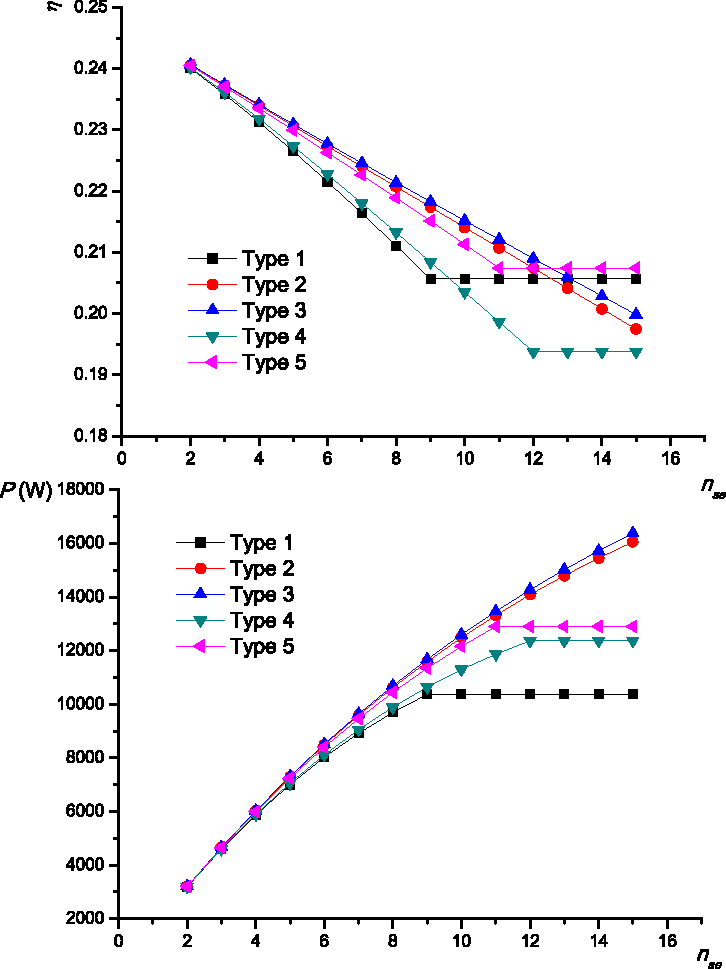
\includegraphics[width = 0.7\columnwidth]{fig/n_se}
	\caption{Influence of $n_{se}$ on efficiency and power of SEA}
	\label{fig:n_se}
\end{figure}

For a certain connection type, increase $n_{se}$ will reduce the efficiency of SEA. For some connection types, increase $n_{se}$ will reduce the output power $P$ due to inoperative engines and smaller output power engines. It is important to choose the number of engines for some connection types of SEA. 

For Type 1, when $n_{se} \geqslant 10$, all engines stop working for given heating and cooling fluids due to small $\dot{m}c_p$. For Type 2 and Type 3, every engine in the SEAs works. $\eta$ reduces with increasing $n_{se}$ due to smaller temperature difference of the fluids, and $P$ increases due to more operating engines. For Type 4, by checking results, it can be found that when $n_{se} = 13$,  the last engine doesn't work; when $n_{se} = 14$, only the first 10 engines will work; when $n_{se} = 15$, the working engine number drops to 9. For Type 5, by checking results, it can be found that when $n_{se} = 12$, the last 2 engines stop working; when $n_{se} = 13$, only the first 8 engines will work; when $n_{se} = 14$, the working engine number drops to 6; when $n_{se} = 15$, the working engine number drops to 4. The aforementioned strategy is applied to achieve maximum total output power. For Type 4, when $n_{se} \geqslant 13$, the number of the operating engines is changed to be 12 to achieve maximum output power. For Type 5, when $n_{se} \geqslant 12$, the number of the operating engines is changed to be 11 to achieve maximum output power.
Horizontal lines in \autoref{fig:n_se} shows the application results of the strategy. 

\section{Conclusion}

%A new layout scheme of the solar dish system by using SEA are proposed in this thesis. 
Connection type of the engines changes the flow rates and temperatures of the fluids, as a result the performance of the SEA will be different depending on the connection schemes. In order to compare performance of SEAs with different arrangements, five basic connection types of SEA are classified according to flow type and flow order. 

%Analytical Stirling engine model is created to develop the SEA models for the investigation of influence of connection types. Imperfect regeneration and cycle irreversibility of Stirling engine cycle and heat exchange process between fluids and engine are considered in the model. Algorithm to numerically solve different connection types of SEA is developed. The model is evaluated by considering the prototype GPU-3 Stirling engine as a case study. Result shows that the proposed model predicted the performance with higher accuracy than Simple model~\cite{Urieli1984} and Simple II model~\cite{Strauss2010}. 

Models of different connections of SEAs are developed to investigate the performance under different parameters and the impacts of $T_{i,h}$, $\dot{m}_hc_{p,h}$, $\dot{m}_cc_{p,c}$ and $n_{se}$ with different connection types. It is found that

\begin{enumerate}[label=(\arabic*)]
\item Reduce $T_{i,h}$ or $\dot{m}c_{p}$ will weaken the performance of SEA of all connection types. This is obvious since lower $T_{i,h}$ or $\dot{m}c_p$ leads to lower temperature distribution of the hot chamber of the Stirling engines. Lower temperature difference of the hot chamber and cold chamber leads to lower efficiency.
\item When inlet temperature of hot fluid ($T_{i,h}$) is lower than a critical value, some engines in the SEAs will stop working. Reduce the number of operating engines may help for the total output power.
\item Different connection types of SEAs show different adaptability for low $T_{i,h}$. Type 2 shows the best adaptability for low $T_{i,h}$. when $T_{i,h} \geqslant 730\,\mathrm{K}$, all the 6 engines are running.
\item SEA of serial flows (Type 3) has the best performance and adaptability under different parameters. Given heating and cooling fluids, using serial flow is the best choice for the connection type of an SEA.
	
\end{enumerate}